\documentclass[xcolor=dvipsnames]{beamer}

\usetheme{Boadilla}

\newcommand{\bi}{\begin{itemize}}
\newcommand{\ei}{\end{itemize}}
\newcommand{\be}{\begin{enumerate}}
\newcommand{\ee}{\end{enumerate}}
\newcommand{\I}{\item}
\newcommand{\f}{\frame}
\newcommand{\ft}{\frametitle}

\title{Overview of Requirements}
\subtitle{for the FDC Mini-Review}
\author[M.\ Ito]{Mark M.\ Ito}
\date{February 1, 2008}
\institute[JLab]{Jefferson Lab}

\begin{document}

\f{\titlepage}

\f{
  \ft{Outline}
  \bi
  \I physics goals
  \I GlueX detector
  \I reviews: past, present and future
  \I design considerations
  \I performance
  \I conclusions
  \ei
}

\f{
  \centerline{\Large physics goals}
}
\f{
  \ft{goals and requirements}

  Map the spectrum of hybrid mesons (gluonic excitations)
    \bi
    \I Start search with those with exotic quantum numbers
    \I Make contact with spectroscopy of non-exotic states
    \ei
\begin{columns}[c]
  \begin{column}{2in}
  Analysis will require
    \bi
    \I partial-wave analysis
    \I identification of exclusive final states
    \I detailed understanding of backgrounds
    \I large event samples
    \I confirmation of states in multiple decay channels
    \ei
  \end{column}
  \begin{column}{2in}
$$
  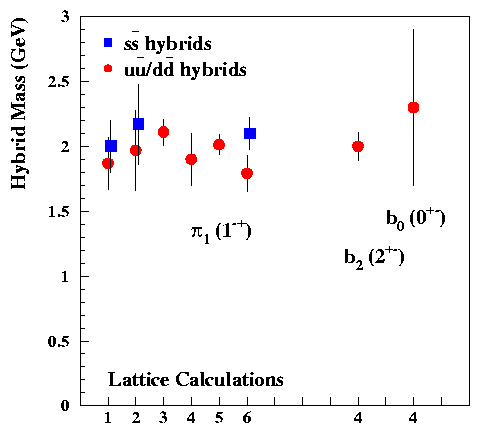
\includegraphics[height=1.5in]{hybrids_lattice.png}
$$
  lattice mass predictions
  \end{column}
\end{columns}
}

\f{
  \ft{representative kinematics}
  \onslide<1->{
    \bi
    \I $t$-channel meson photoproduction: $\sigma(t)\propto e^{\beta t}$, $\beta = 5$~GeV$^{-2}$
    \I $\gamma$ incident with 8-9~GeV
    \I exclusive kinematics
    \ei
  }
  \only<1>{
    \begin{columns}[c]
      \begin{column}{1.0in}
        pions
        \bi
        \I $p < 5$~GeV
        \I $\theta < 20^\circ$
        \ei
      \end{column}
      \begin{column}{2.5in}
        $$
        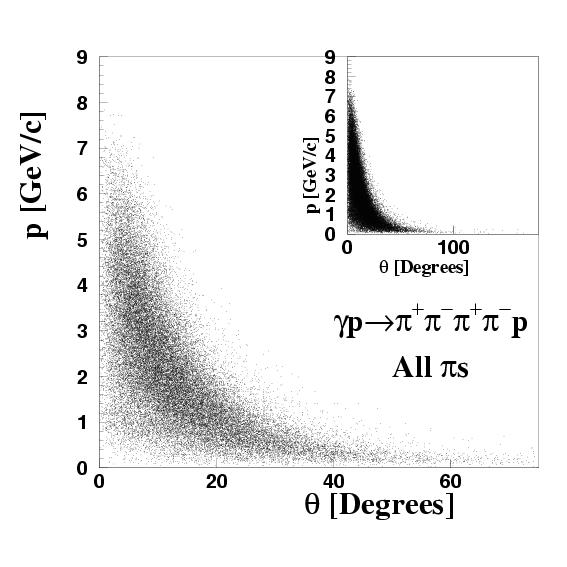
\includegraphics[height=2.5in]{pion_kinematics.jpg}
        $$
      \end{column}
    \end{columns}
  }
  \only<2>{
    \begin{columns}[c]
      \begin{column}{1.0in}
        protons
        \bi
        \I $p < 1$~GeV
        \I $10^\circ < \theta < 60^\circ$
        \ei
      \end{column}
      \begin{column}{2.5in}
        $$
        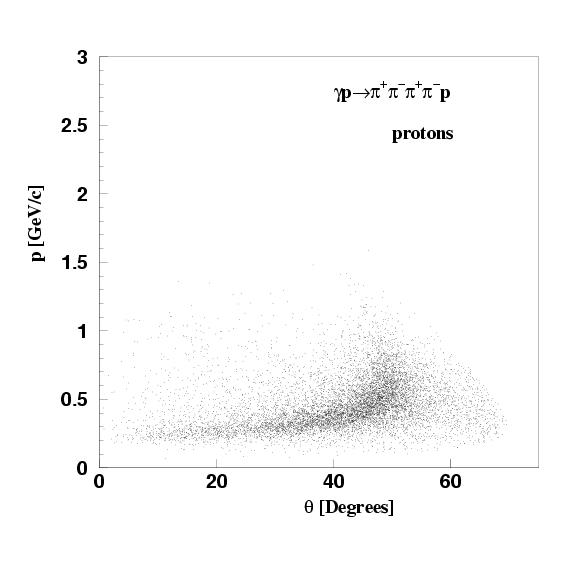
\includegraphics[height=2.5in]{proton_kinematics.jpg}
        $$
      \end{column}
    \end{columns}
  }
  \only<3>{
    \begin{columns}[c]
      \begin{column}{1.0in}
        photons
        \bi
        \I $p < 4$~GeV
        \I $\theta < 60^\circ$
        \ei
      \end{column}
      \begin{column}{2.5in}
        $$
        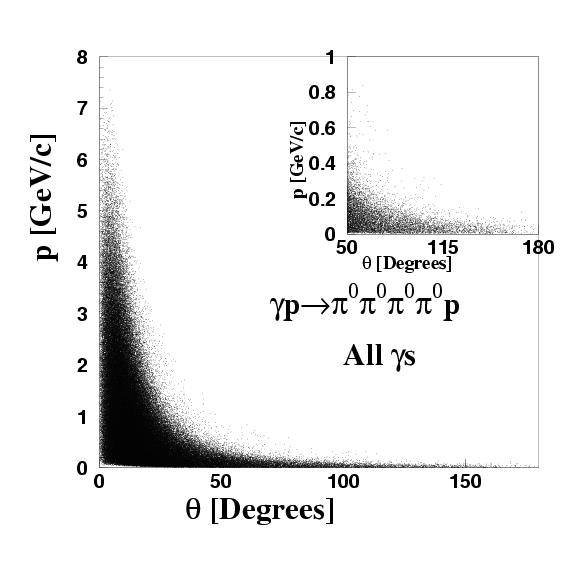
\includegraphics[height=2.5in]{photon_kinematics.jpg}
        $$
      \end{column}
    \end{columns}
  }
}

\f{
  \ft{anything else?}
  \bi
  \I Hall D a unique facility
    \bi
    \I 9~GeV tagged photon beam
    \I coherent bremsstrahlung $\Rightarrow$ nearly mono-energetic beam
    \I linear polarization
    \ei
  \I driven to a general purpose detector
    \bi
    \I charged and neutral particle detection
    \I very large acceptance
    \ei
  \I other physics possible!
    \bi
    \I come to the workshop, PHP2008, March 6-8, at JLab
    \I ``Photon-hadron physics with the GlueX detector at Jefferson Lab''
    \ei
  \ei
}
\f{
  \centerline{\Large GlueX detector}
  $$
  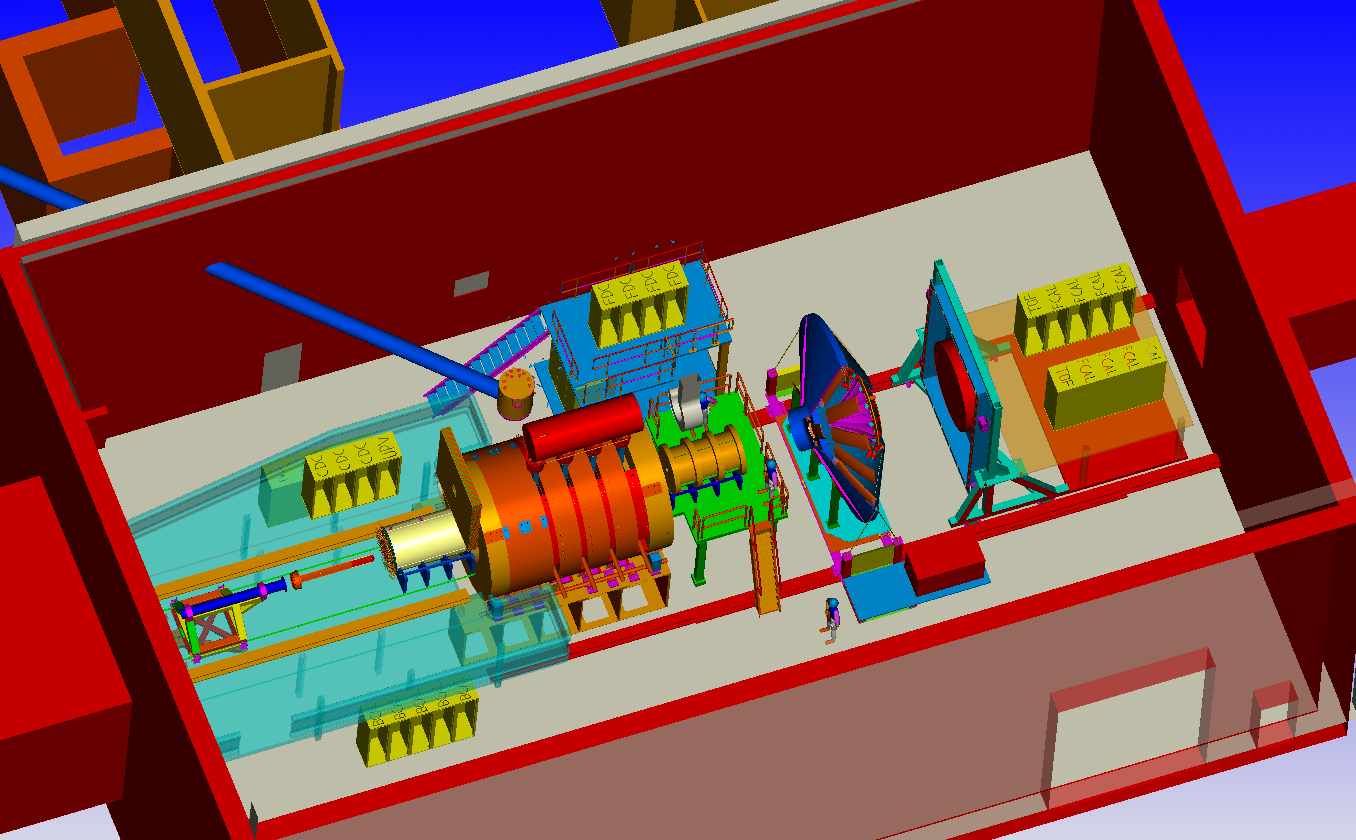
\includegraphics[height=2.9in]{gluex_in_hall_d.png}
  $$
}
\f{
  \ft{elevation view}
  $$
  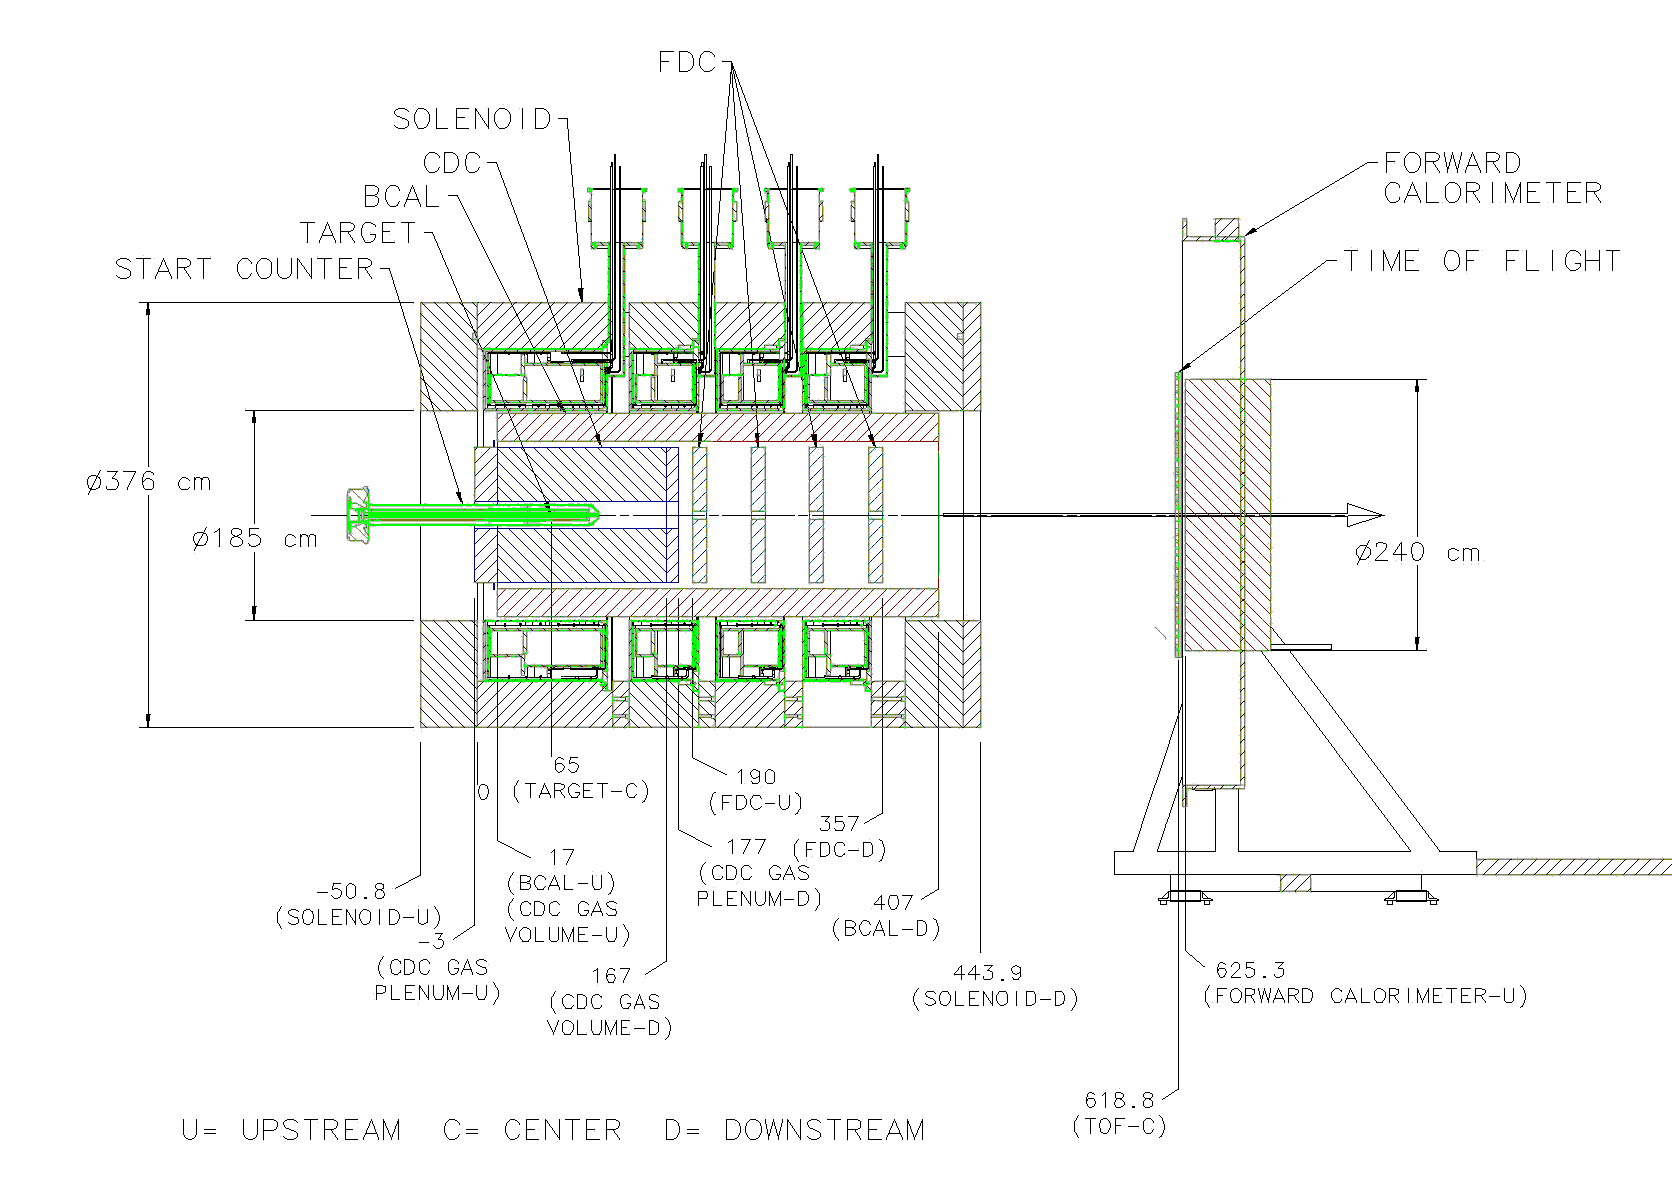
\includegraphics[height=2.9in]{gluex_detector.png}
  $$
}
\f{
  \centerline{\Large reviews: past, present and future}
}
\f{
  \ft{review schedule}
  \bi
  \I \textcolor{red}{Drift Chamber Preliminary Design Review, Hall B and D, March 2007}
  \I CD-2 12 GeV Project Review, June 2007
  \I
  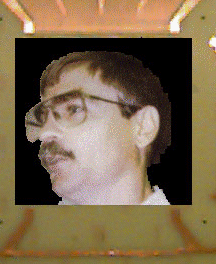
\includegraphics[height=0.5in]{howard_pwc.png}\textcolor{red}{$\leftarrow$FDC
    Mini-Review, February
    2008$\rightarrow$}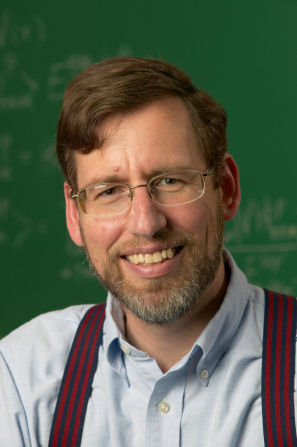
\includegraphics[height=0.5in]{Larry_Weinstein.jpg}
  \I \textcolor{red}{Drift Chamber Final Design Review, March 2008}
  \I CD-3 Project Review, July 2008
  \ei
}
\f{
  \ft{Drift Chamber Review, Hall B and D, March 2007}

  Comment (excerpted)

  \bi
  \I In preparation for future reviews, the collaboration should
  better articulate how the performance requirements of the tracking
  detectors are derived from the goals of the experimental program.
  \ei

  Recommendations (complete)

  \begin{enumerate}

    \I Priority should be given to studying design modifications that
    would significantly reduce the amount of material in the GlueX
    tracking chambers.

    \I Additional resources and expertise should be applied to the
    development of track reconstruction software for GlueX, and to a
    complete and realistic hit-level simulation of the GlueX
    spectrometer.

  \end{enumerate}
}

\f{
  \centerline{\Large design considerations}
}
\frame<1-3>[label=general-stuff]{
  \ft{really general stuff}
  \bi
  \item<alert@1> characteristics of the acceptance
    \bi
    \I must be large
    \I must be smooth
    \I must be well understood
    \I driven by need to do a partial-wave analysis
    \ei
  \I<alert@2> resolution counts
    \bi
    \I needed for missing mass identification
    \I reduces combinatoric background under narrow resonances
    \I sharpens results from the partial-wave analysis
    \I surprises, unintended benefits, etc.
    \ei
  \I \alert<3,4>{low mass counts}
    \bi
      \I<alert@3> reduce multiple scattering contribution to resolution
      \I<alert@4> reduce production of secondaries (especially photon conversions)
    \ei
  \I<alert@5> robust pattern recognition
    \bi
    \I robustness $\Leftrightarrow$ simplicity $\Leftrightarrow$
    speed of reconstruction
    \ei
  \ei
}

\f{
\ft{material reduction program}
\small
\begin{tabular}{|llrrr|}
\hline
&&& Mar.\ '07 & Feb.\ '08 \\
Layer & Material & Density	(g/cm$^3$) & \multicolumn{2}{c|}{$x/X_0$} \\
\hline
Ground	plane & mylar & 1.3900 & 0.00000 & 0.00000 \\
Rohacell & Rohacell & 0.0320 & 0.00039 & 0.00016 \\
Cathode & epoxy & 1.0000 & 0.00006 & 0.00005 \\
Cathode & Kapton & 1.4200 & 0.00017 & 0.00009 \\
Cathode & Cu & 8.9600 & 0.00035 & 0.00014 \\
Gas & Ar/CO2 & 0 & 0.00007 & 0.00007 \\
Wires sense & W & 0 & 0.00001 & 0.00001 \\
Wires field & Al & 0 & 0.00001 & 0.00001 \\
Cathode & Cu & 8.9600 & 0.00035 & 0.00014 \\
Cathode & Kapton & 1.4200 & 0.00017 & 0.00009 \\
Cathode & epoxy & 1.0000 & 0.00006 & 0.00005 \\
Rohacell & Rohacell & 0.0320 & 0.00039 & 0.00016 \\
\hline				
Thickness per plane &&& 0.00204 & 0.00095 \\
Thickness per package &&& 0.01224 & 0.00569 \\			
Thickness for 4 packages &&& 0.04897 & 0.02276 \\
\hline
\end{tabular}
}

\againframe<4>{general-stuff}

\f{
  \ft{photon conversions}
  \onslide<1->{
    \centerline{photon conversion points, minimum bias events (PYTHIA)}
  }
  \only<1>{
    $$
    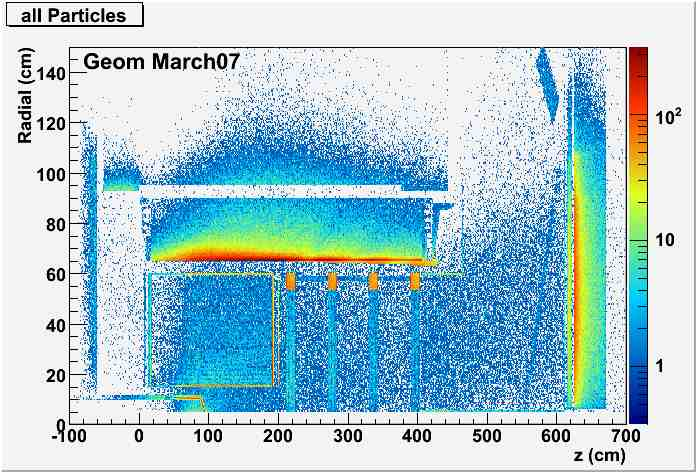
\includegraphics[height=2.0in]{all_particles_stop_A_geommarch07.jpg}
    $$
    \centerline{March 2007 Geometry, dual cathode FDC,
      frame $\rightarrow$ $76\% of X_0$}
  }
  \only<2>{
    $$
    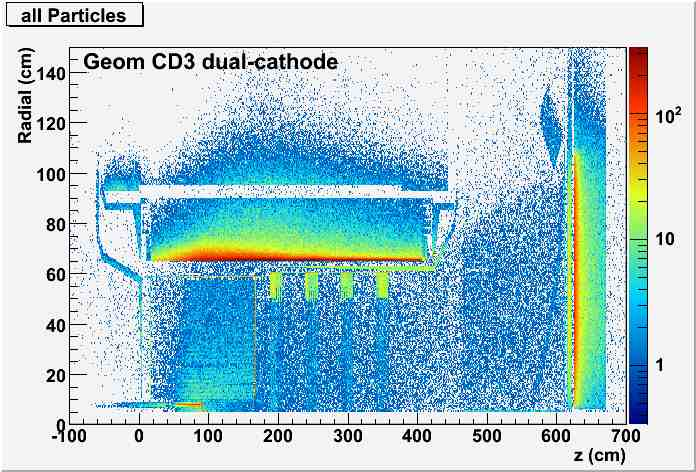
\includegraphics[height=2.0in]{all_particles_stop_A_geomcd3dualcathode.jpg}
    $$
    \centerline{February 2008 Geometry, dual cathode FDC,
      frame $\rightarrow$ $39\% of X_0$}
  }
}

\againframe<5>{general-stuff}

\f{
\ft{event display}
\begin{columns}[t]
  \begin{column}{1.2in}
    FDC reconstruction particularly challenging
    \bi
    \I many forward going tracks
    \I possible ambiguities correlating layers
    \ei
  \end{column}
  \begin{column}{3.0in}
    $\gamma p \rightarrow \pi^+ \pi^- \pi^+ \pi^- p$ \\
    \hspace{0.15in} via $\gamma p \rightarrow \eta_c p$ \\
    \hspace{0.30in} $\eta_c \rightarrow \rho^0 \rho^0$ \\
    \hspace{0.45in} $\rho^0 \rightarrow \pi^+\pi^-$ \\
    $$
    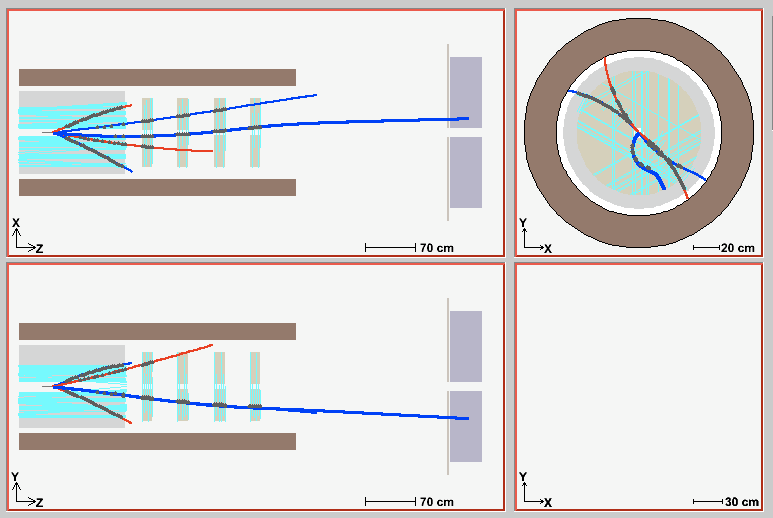
\includegraphics[width=3.0in]{event_display.png}
    $$
  \end{column}
\end{columns}
}

\f{
  \ft{background zoology}
  \bi
    \I electronic noise $\rightarrow$ isolated hits
    \I e\&m $\rightarrow$ isolated hits and tracks
    \I hadronic $\rightarrow$ non-signal physics events
    \I combinatoric $\rightarrow$ false decay particle attribution
  \ei
}

\f{
  \ft{common features of all FDC options}
  \begin{columns}[c]
    \begin{column}{2.5in}
        \bi
        \I drift chambers and/or cathode strip chamber technology
        \I no structural segmentation in azimuth (no $\phi$ sectors)
        \I pipeline readout
        \I variations on design work already done for the default dual-cathode design  
        \ei
    \end{column}
    \begin{column}{1in}
      $$
      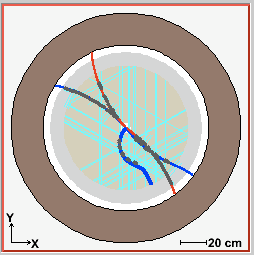
\includegraphics[width=1.0in]{event_display_zview.png}
      $$
    \end{column}
  \end{columns}
}
\f{
  \ft{default design}

  two cathode strip planes per wire plane (dual-cathode design)
    \bi
    \I six anode wire planes per package
    \I twelve cathode strip planes
    \I cathodes at $\pm 75^\circ$
    \I each anode plane rotated $60^\circ$ from previous anode plane
    \I TDC readout for anodes
    \I FADC readout for cathodes
    \ei
}
\f{
  \ft{alternate design options}
  \be
    \I no cathode strips (wires-only design)
    \bi
      \I twelve anode wire planes per package
      \I orientation options:
      \be
        \I each plane rotated $60^\circ$ from previous (subject of studies)
        \I pairs of planes with half-cell offset, pairs rotated
        $60^\circ$ from previous
      \ee
    \ei
    \I one cathode strip plane per anode wire plane (single-cathode design)
  \ee
}
\frame<1->[label=pros-cons]{
  \ft{\textcolor{ForestGreen}{pro's} and \textcolor{red}{con's}}
  \bi
  \I two-cathode design
    \be
      \I \textcolor{ForestGreen}{position resolution of cathodes in a layer good enough to select single wire in anode plane}
      \I \textcolor{ForestGreen}{cathodes strips and anode wires see the same avalanche}
      \bi
        \I \textcolor{ForestGreen}{can use timing to correlate strips with wires}
        \I \textcolor{ForestGreen}{FADC's on cathode strips give a time measurement}
        \I \textcolor{ForestGreen}{time resolution should be sufficient}
        \I \textcolor{ForestGreen}{especially useful in eliminating isolated single-cell hits}
      \ei
    \I \textcolor{red}{Lorentz effect introduces L-R ambiguity in cathode strip information}
    \ee
  \I wires-only design
    \be
    \I \textcolor{ForestGreen}{cathode strip planes replaced with thin cathode sheets; much less material}
    \I \textcolor{ForestGreen}{cost savings due to fewer electronics channels and/or replacement of FADC's with TDC's}
    \I \textcolor{red}{puts pressure on pattern recognition because of crossing ambiguities}
    \ee
  \ei
}

\f{
  \ft{Lorentz effect}
  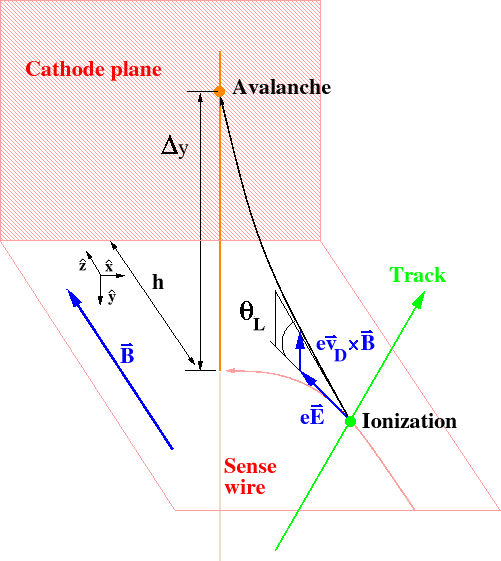
\includegraphics[height=1.9in]{Lorentz_effect.png}
  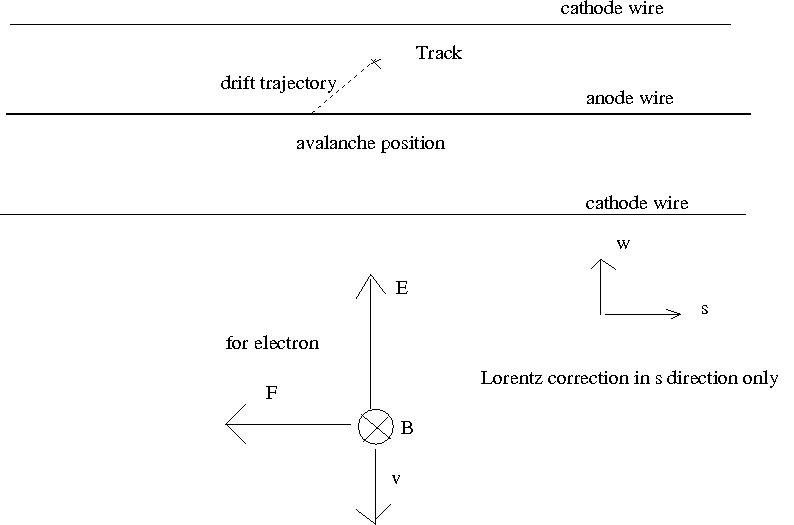
\includegraphics[height=1.9in]{FDC_cell.jpg}
  \bi
    \I cathodes image avalanche
    \I avalanche displaced from ionization location in dimension along anode
    wire
    \I sign of displacement goes as the left-right choice
  \ei
}

\againframe<1>{pros-cons}

\f{
  \centerline{\Large performance}
}

\f{
\ft{benchmark study}
\small
two conventional reactions simulated
\begin{equation}
\gamma p \rightarrow X^+ n \rightarrow \pi^+\pi^+\pi^-n
\end{equation}
\begin{equation}
\gamma p \rightarrow Y^+ n \rightarrow \pi^+\pi^0\pi^0n \rightarrow \pi^+\gamma\gamma\gamma\gamma n
\end{equation}
with appropriate resonant sub-structure
\begin{columns}[t]
\begin{column}{2.2in}
\bi
\I 200~k events accepted in each reaction (a few weeks of running at turn on)
\I detector response simulated
\I partial-wave analysis performed
\I exotic signal searched for
\I none found (good!) at the 1\% level
\ei
\normalsize
FDC: \textcolor{blue}{$\sigma=150~\mu$m, $x/X_0=1.7\%$}
\end{column}
\begin{column}{2.0in}
$$
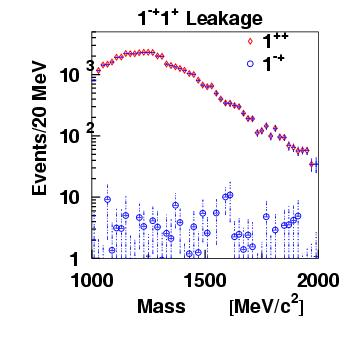
\includegraphics[width=2.0in]{leakage.jpg}
$$
\end{column}
\end{columns}

}

\f{
  \ft{momentum resolution: $\sigma_{p_t}/p_t$ for various designs}
\begin{columns}[t]
  \begin{column}{1.8in}
  \bi
  \I dual-cathode design assumes 24 wire planes + 48 cathode planes
  \I wires-only design assumes 48 measurement planes
  \I<2-> dual cathode, 3 packages: drops one package, overall $z$-distance preserved
  \I<2-> single cathode: drop one cathode plane, 24 wire, 24 cathodes
  \ei
  \end{column}
  \begin{column}{2.8in}
    \only<1>{
      $$
      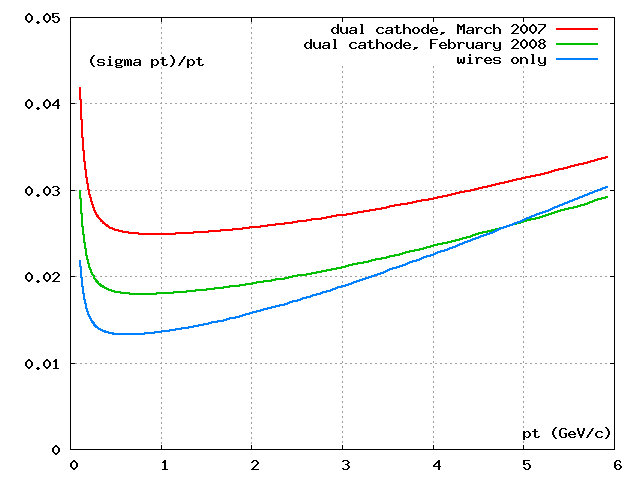
\includegraphics[width=2.8in]{FDC_resolution_partial.png}
      $$
    }
    \only<2>{
      $$
      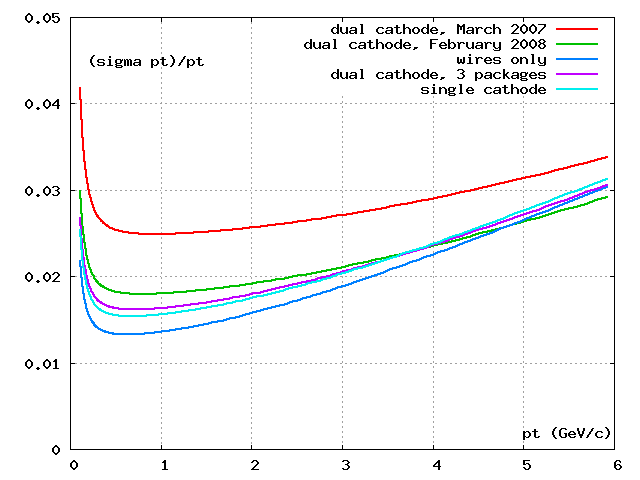
\includegraphics[width=2.8in]{FDC_resolution.png}
      $$
    }
  \end{column}
\end{columns}
}

\f{
\ft{comparison of options}
\begin{center}
\small
\begin{tabular}{|lrrrr|}
\hline
& \# meas & \# meas & $\sigma_x$ & $X_0$ \\
design & anode & cathode & ($\mu$m) & (\%) \\
\hline
dual cathode, Mar.\ '07           & 48 & 24 & 200 & 5.50 \\
dual cathode, Feb.\ '08 (default) & 48 & 24 & 200 & 2.83 \\
dual cathode, 3 pkgs.             & 36 & 18 & 200 & 2.26 \\
single cathode                    & 24 & 24 & 200 & 2.03 \\
wires only                        &  0 & 48 & 200 & 1.49 \\
\hline
\end{tabular}
\end{center}
}

\f{
  \centerline{\Large conclusions}
}
\f{
  \ft{concluding remarks}
  \bi
  \I Material has been reduced significantly since March 2007
    \bi
    \I active volume: $1.4 \rightarrow 0.6\%$ $X_0$
    \I beam area: $1.4 \rightarrow 0.2\%$ $X_0$
    \I frames and support: $76 \rightarrow 39\%$ $X_0$
    \ei
  \I Design very far advanced: Dan's talk
  \I Prototype has been tested: Simon's talk
  \I Reconstruction software coming online: David's talk
  \I Full-scale prototype is on the way
  \I Variations on wire/cathode arrangement still possible without
  additional major engineering effort
  \I Need unambiguous configuration for March 2008 Drift Chamber Review
  \ei
}

\end{document}

%%% end of latex file %%%%
